\documentclass{article}
\usepackage[utf8]{inputenc}
\usepackage[T1]{fontenc}
\usepackage{graphicx}
\usepackage{hyperref}
\usepackage{geometry}
\geometry{margin=1in}

\title{EXEGETION}
\date{Encyclopaedia Britannica (1771)}

\begin{document}
\maketitle

\section*{Historical source}
\textbf{Entry ID:} \texttt{entry-exegetion-1805} \\
\textbf{Volume ID:} 191320560 \\
\textbf{Character Count:} 178

\subsection*{Extracted Text}
EXEGETION, in \_Idyldek\_, the size of finding, eti-ties in numbers or lines, the roots of the equation of the problem, according as the problem is either numerical or promotional.



\section*{Source record}
\begin{itemize}
\item \textbf{Dataset:} \texttt{NationalLibraryOfScotland/encyclopaedia\_britannica\_illustrated}
\item \textbf{Dataset Revision:} \texttt{309f765b1ecc83e0a7f7762e44b4a927a7555443}
\item \textbf{Page ID:} \texttt{britannica:309f765b1ecc83e0a7f7762e44b4a927a7555443:train:1805} \\
  \textbf{Filename:} \texttt{page-1805-226885408318.jpg} \\
  \textbf{Row Index:} 1805 \\
  \textbf{SHA256:} \texttt{2268854083181b93...}
\end{itemize}

\begin{figure}[h]
\centering
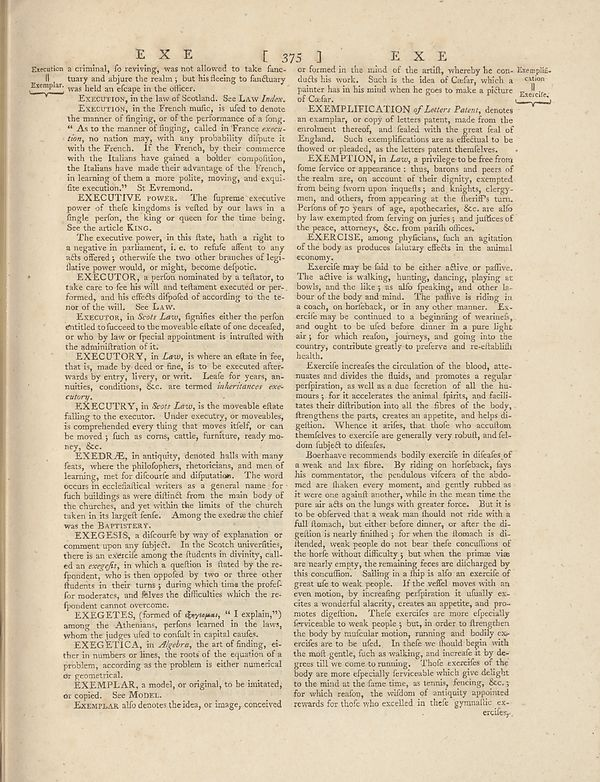
\includegraphics[width=0.85\textwidth]{../scans/page-1805-226885408318.jpg}
\caption*{Source scan: \texttt{page-1805-226885408318.jpg}}
\end{figure}

\end{document}
